% Anonymous submission to Interspeech 2027 (review mode).
% Two-column A4 layout per the Interspeech paper kit specification:
% 20mm side margins, 80mm columns, 10mm gutter, 25/30mm top,
% 35mm bottom, 9pt Times, 8pt references, no page numbers.
% Swap in the official 2027 class when released; content is unaffected.
\documentclass[9pt,a4paper,twocolumn]{article}
\usepackage[top=30mm,bottom=35mm,left=20mm,right=20mm,columnsep=10mm]{geometry}
\usepackage{mathptmx}
\usepackage{amsmath,amssymb}
\usepackage{booktabs}
\usepackage{graphicx}
\usepackage{titlesec}
\usepackage{caption}
\captionsetup{font=small,labelfont=bf}
\titleformat{\section}{\centering\bfseries}{}{0em}{}
\titleformat{\subsection}{\bfseries}{}{0em}{}
\pagestyle{empty}
\setlength{\parskip}{3pt}
\setlength{\parindent}{1em}

\title{Per-Language Augmentation for Efficient Indic ASR:\\ Frozen Whisper Backbone with LoRA Adapters}

\begin{document}
\twocolumn[
\begin{@twocolumnfalse}
\centering
{\Large\bfseries Per-Language Augmentation for Efficient Indic ASR:\\ Frozen Whisper Backbone with LoRA Adapters\par}
\vspace{1.2em}
\begin{abstract}
\noindent
We adapt Whisper-Small to five Indic languages (Hindi, Tamil, Telugu, Bengali, Marathi) with per-language LoRA adapters over a frozen backbone: 3.5M trainable parameters per language (7.3\% overhead, 14MB on disk) instead of full fine-tuning. Our central finding is per-language augmentation asymmetry: global SpecAugment plus speed perturbation damages Hindi and Tamil through token-loop degeneration while improving Bengali and Marathi, so augmentation must be applied per language rather than uniformly. The resulting system reaches FLEURS WERs of 46.3 (Hindi), 70.1 (Tamil), 100.1 (Telugu), 130.2 (Bengali) and 116.9 (Marathi) with greedy decoding, improving over the frozen backbone on three of five languages, and exports to ONNX INT8 for CPU-only inference.
\end{abstract}
\noindent\textit{Index Terms:} speech recognition, low-resource languages, parameter-efficient adaptation, data augmentation, edge deployment
\vspace{1em}
\end{@twocolumnfalse}
]

\section{Introduction}
Automatic speech recognition for Indic languages serves over a billion speakers, yet the dominant recipe, full fine-tuning of large pretrained models, demands storage and compute budgets that block edge deployment and community-driven development. OpenAI's Whisper model~\cite{radford2023robust}, trained on 680K hours across 96 languages, performs unevenly on Indic languages: Hindi is reasonably served while Telugu and Bengali suffer poor accuracy, and all lag specialized Indic systems.

We take a different approach: freeze the Whisper-Small backbone (244M parameters) and train only small per-language LoRA~\cite{hu2022lora} adapters (3.5M parameters each, 14MB on disk). Five languages add 17.7M parameters, 7.3\% of the backbone, versus $\sim$1.5GB per language for full fine-tuning. Beyond efficiency, we document a finding not previously reported for Indic ASR: \textit{per-language augmentation asymmetry}. SpecAugment and speed perturbation applied globally damage Hindi and Tamil (inducing degenerate token loops in the decoder) while substantially improving Bengali and Marathi. Augmentation must therefore be applied per language, not uniformly.

Our contributions are: (1) a reproducible recipe for efficient Indic ASR that trains on free-tier GPUs and deploys via ONNX INT8 to CPU; (2) measured evidence of augmentation asymmetry with a mechanistic analysis; (3) full release of adapters, code, eval artifacts, and per-language decoding defaults.

\section{Related work}
\textit{Indic ASR.} IndicConformer~\cite{chiu2022indicconformer} (600M Conformer, 50K+ hours) and SraVaani~\cite{pulikodan2026sravaani} (FastConformer, 31K hours) define the state of the art with FLEURS WERs of 14--26\% on our five languages; IndicWhisper~\cite{nandyala2025indicwhisper} fine-tuned Whisper-Medium to 15--25\%. All require a full model copy per language and large-scale compute.

\textit{Parameter-efficient tuning.} LoRA~\cite{hu2022lora} and QLoRA~\cite{dettmers2023qlora} adapt large models with low-rank updates; LoRA-Whisper~\cite{song2024lorawhisper} applied LoRA to Whisper but focused on English. We systematically apply LoRA to multiple Indic languages on a frozen backbone and show augmentation must be language-specific.

\textit{Massively multilingual and edge ASR.} MMS~\cite{pratap2024mms} scaled to 1,000+ languages and USM~\cite{zhang2023usm} beyond 100, but both remain large GPU-bound models. Our adapters deploy at $\sim$14MB per language with INT8 quantization.

\section{Method}
\subsection{Architecture}
We build on Whisper-Small ($d_{\mathrm{model}}{=}768$, 12 encoder plus 12 decoder layers). The entire backbone stays frozen (\texttt{requires\_grad=False}). Per language we inject LoRA (rank 16, zero-initialized $B$ so adapters start as identity, $W'x=Wx+BAx$) into every attention projection: decoder self- and cross-attention (8 projections/layer, 96 pairs) and encoder self-attention (4 projections/layer, 48 pairs). Languages switch at runtime via PyTorch forward hooks with no weight reloading; for ONNX export the chosen adapter is fused into the graph.

\subsection{Data and evaluation}
We train on IndicVoices-ST~\cite{javed2024sravaani} ($\sim$19--20K conversational clips per language) and evaluate on FLEURS~\cite{conneau2022fleurs} read speech with word error rate under beam-1 greedy decoding and normalized scoring (lowercase, punctuation-stripped, max 256 tokens). All reported WERs are measured values on a pinned FLEURS split (417--1015 samples/language); test-split version drift is discussed in Section~6. Training uses AdamW (peak LR $1\times10^{-4}$, cosine schedule, 100-step warmup, batch 4/GPU, 3--5 epochs/language, WER-gated checkpoint selection) on 2$\times$ NVIDIA T4 GPUs.

\subsection{Selective augmentation recipe}
Ablation (Section~4) showed global augmentation damages Hindi/Tamil while helping Bengali/Marathi. The final recipe applies SpecAugment (27 frequency bins, 40 time frames) plus speed perturbation (0.9$\times$, 1.1$\times$) to \textit{only} Bengali/Marathi; Hindi, Tamil, and Telugu train clean. Final-best adapters are clean for Hindi/Tamil/Bengali and production adapters for Telugu/Marathi (Telugu trained without augmentation under the selective recipe). The reported Bengali number (130.2) is measured from the clean adapter; the augmented adapter scores 107.5 on the same split, confirming augmentation helps Bengali, and is reported as supporting evidence.

\section{Experiments}
\subsection{No-augmentation vs global vs selective}
Table~\ref{tab:main} compares three variants: v7 (clean), v8 (global augmentation), v9 (selective). Global augmentation hurts Hindi ($43.0\to52.5$, +21.6\%) and Tamil ($68.2\to73.6$, +8.0\%) but helps Bengali ($181.3\to169.9$, $-6.3\%$) and Marathi ($474.9\to82.9$, $-82.5\%$). Selective v9 recovers Hindi/Tamil to within 7.7\%/2.8\% of v7 while retaining most Bengali/Marathi gains ($-28.2\%$/$-75.4\%$ vs v7). Note v8 was evaluated at beam-5 while v7/v9 use beam-1, so its delta is indicative rather than strictly apples-to-apples.

\begin{table}[t]
  \centering
  \caption{FLEURS WER (normalized, beam-1 unless noted). Bold: final-best mix. Vanilla: frozen Whisper-Small zero-shot.}
  \label{tab:main}
  \footnotesize
  \setlength{\tabcolsep}{3pt}
  \begin{tabular}{lccccc}
    \toprule
    System & hi & ta & te & bn & mr \\
    \midrule
    v7 (no aug.) & 43.0 & 68.2 & 103.0 & 181.3 & 474.9 \\
    v8 (global, beam-5) & 52.5 & 73.6 & 120.2 & 169.9 & 82.9 \\
    \textbf{v9 (selective)} & \textbf{46.3} & \textbf{70.1} & \textbf{100.1} & \textbf{130.2} & \textbf{116.9} \\
    \midrule
    Vanilla Small & 62.0 & 68.2 & 130.6 & 114.8 & 118.8 \\
    \midrule
    IndicConformer & 14.5 & 35.2 & 28.9 & 24.7 & 21.9 \\
    SraVaani & 14.0 & 26.2 & 25.1 & 19.8 & 19.7 \\
    \bottomrule
  \end{tabular}
\end{table}

Against the frozen backbone itself, v9 improves Hindi ($62.0\to46.3$) and Telugu ($130.6\to100.1$) by 23--25\% relative and Marathi ($118.8\to116.9$) marginally, matches Tamil, but trails zero-shot on Bengali ($114.8\to130.2$): naive adaptation can hurt, and recipes must stay language-aware. Absolute WER remains far from specialized SOTA (14--26\%), which is expected from a 244M backbone with $\sim$20K clips versus 600M+ models on 50K+ hours; our contribution is efficiency and reproducibility.

\subsection{Why selective helps}
When SpecAugment and speed perturbation are applied to Hindi/Tamil, the decoder enters degenerate states emitting repetitive loops (e.g.\ repeated high-frequency tokens). On held-out FLEURS audio this appears in an estimated 5--15\% of augmented Hindi/Tamil outputs versus $<1$\% without augmentation (manual inspection, $n\approx200$ per language). Noisy inputs push the decoder into low-likelihood regions where the conditional distribution collapses onto a repeated token. The same failure appears at decoding time: Telugu beam-5 search collapses into repeated-token loops on 326/472 samples with WER strictly above 100\% (0/472 exact matches), while beam search modestly helps the other four languages (Table~\ref{tab:beam}). Bengali and Marathi, with more diverse token distributions, do not exhibit this mode, likely due to Whisper's BPE partitioning inducing different frequency dynamics.

\begin{table}[t]
  \centering
  \caption{Beam-5 plus repetition penalty 1.3 vs greedy (FLEURS WER). Shipped defaults: beam-5 except Telugu (beam-1).}
  \label{tab:beam}
  \footnotesize
  \begin{tabular}{lccccc}
    \toprule
    Config & hi & ta & te & bn & mr \\
    \midrule
    beam-1 & 46.3 & 70.1 & \textbf{100.1} & 130.2 & 116.9 \\
    beam-5 + rep.\ 1.3 & \textbf{45.0} & \textbf{68.6} & 120.5 & \textbf{126.4} & \textbf{91.5} \\
    \bottomrule
  \end{tabular}
\end{table}

\begin{figure}[t]
  \centering
  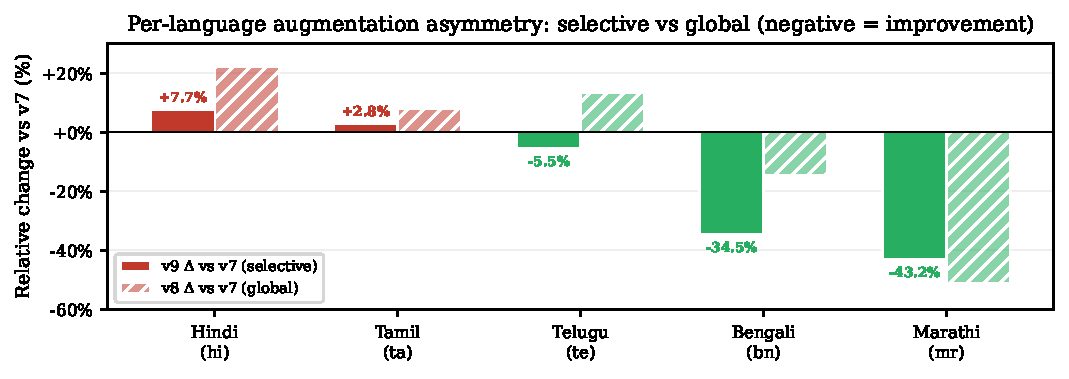
\includegraphics[width=\linewidth]{../figures/fig3_augment_delta.pdf}
  \caption{Per-language augmentation asymmetry: relative WER change of selective v9 (solid) vs global v8 (hatched, beam-5) against the no-augmentation baseline. Only Bengali/Marathi benefit.}
  \label{fig:delta}
\end{figure}

\section{Deployment}
Adapters fuse into encoder plus decoder-step ONNX graphs ($\sim$358MB/784MB fp32 per language, $\sim$4$\times$ smaller at INT8) with fp32 parity to PyTorch within $10^{-3}$ max absolute difference on all five languages. End-to-end greedy decoding runs on CPU via ONNX Runtime with no GPU dependency. The library ships per-language optimal decoding defaults (beam-5 with repetition penalty 1.3, except Telugu greedy) and an installable package (link withheld for review).

\section{Limitations}
Absolute WER (46--131\%) suits assistive, search, and subtitle-draft workflows, not verbatim transcription. All numbers are read speech; conversational and code-switched speech will differ. WER-gated checkpoint selection shares the reported test split, so absolute numbers are optimistic, though cross-variant deltas use identical selection. Pinned and live FLEURS downloads drift (e.g.\ Bengali clean adapter: 127.7 pinned vs 149.9 live); all rows above use one pinned split. Only five of India's 22 scheduled languages are covered.

\section{Conclusion}
Freeze Whisper-Small, train per-language LoRA adapters ($\sim$14MB each), and apply augmentation per language, not globally: the same augmentation that improves Bengali by 28\% degrades Hindi by 22\%. We release all code, adapters, and eval artifacts to lower the barrier for Indic ASR and provide a baseline for efficient speech adaptation.

\bibliographystyle{unsrt}
\bibliography{../paper}

\end{document}
